% !TEX TS-program = XeLaTeX
%to run:
%xelatex thesis.tex
%bibtex thesis.tex
%xelatex thesis.tex
%xelatex thesis.tex

%Thesis template for M.Sc. degree
\documentclass[12pt,oneside]{report}
\usepackage[a4paper,right=3cm,top=3cm,left=2.5cm,bottom=2.5cm]{geometry}
\renewcommand{\baselinestretch}{1.15}

\usepackage[pdfauthor={نام نویسنده},
            pdftitle={عنوان تر},
            pdfsubject={موضوع},
            pdfkeywords={واژگان کلیدی},
            colorlinks=true]{hyperref}

%اضافه کردن فهرست اشکال و جداول و کتاب‌نامه به فهرست مطالب
\usepackage[nottoc]{tocbibind}
%برای ارائه سورس‌کد در متن
\usepackage{listings}
%برای استفاده از شکل‌های چند بخشی
\usepackage{caption}
\usepackage{subcaption}
%برای روابط ریاضی
\usepackage{amsmath}
%برای جداول بلند
\usepackage{longtable}
%برای استفاده از تصاویر
 %تصاویر در دایرکتوری Figures قرار می‌گیرند.
\usepackage{graphicx}
\graphicspath{{./Figures/}}
%برای شخصی‌سازی شمایل صفحه
\usepackage{fancyhdr}
\pagestyle{fancy}
\fancyhead{}
\rhead{\leftmark}
\lhead{\rightmark}
\fancyfoot{}
\cfoot{\thepage}
%برای ارجاع‌دهی به مراجع
\usepackage[authoryear]{natbib}
\usepackage{amssymb}
\usepackage[localise,extrafootnotefeatures]{xepersian}
\settextfont[Scale=1]{Yas}
\setdigitfont{Yas}

%تعریف دستور برای پانوشت بدون شماره
\newcommand\blfootnote[1]{%
  \begingroup
  \renewcommand\thefootnote{}\footnote{#1}%
  \addtocounter{footnote}{-1}%
  \endgroup
}

\شروع{نوشتار}
\pagenumbering{tartibi}
\title{عنوان پایان‌نامه}
\author{نام}
\date{\today}
%عنوان فارسی
\begin{titlepage}
\vspace*{1cm}
\begin{center}
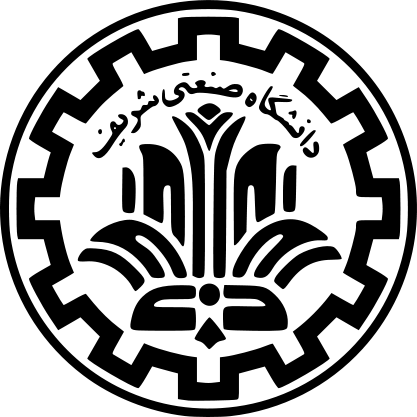
\includegraphics[width=4cm]{sharif.png}

 \large
 دانشگاه صنعتی شریف


دانشکده‌ی مهندسی عمران

\vspace*{1cm}
\large
\textbf{پایان‌نامه به عنوان تحقّق بخشی از شرایط دریافت درجه‌ی کارشناسی ارشد}


\textbf{گرایش مهندسی محیط‌زیست}

\vspace*{1.5cm}
\Huge
\textbf{عنوان تز}     
\vspace{1.5cm}

\Large

نگارش

\textbf{نام دانشجو}
\vspace{1.5cm}

استاد راهنما

\textbf{نام استاد راهنما}
\vfill
\Large
\today        
\end{center}
\end{titlepage}

%تصویب‌نامه
\chapter*{}
\begin{center}
\large
\textbf{\textit{تصویب‌نامه}}\\
\vspace{0.9cm}
\textbf{به نام خدا}\\
\textbf{دانشگاه صنعتی شریف}\\
\textbf{دانشکده‌ی مهندسی عمران}\\
\end{center}
\vspace{0.9cm}

\textbf{پایان‌نامه کارشناسی ارشد}\\

عنوان:
\textbf{عنوان تز}\\

نگارش:
\textbf{نام دانشجو}\\

\vspace{0.9cm}

\textbf{کمیته‌ی داوران}
\vspace{0.9cm}

استاد راهنما:
\textbf{استاد راهنما} \hfill امضاء: ..............................
\vspace{0.9cm}

استاد مشاور:
\textbf{دکتر مشاور} \hfill امضاء: ..............................
\vspace{0.9cm}

ممتحن داخلی:
\textbf{دکتر ممتحن} \hfill امضاء: ..............................
\vspace{0.9cm}

ممتحن داخلی:
\textbf{دکتر ممتحن} \hfill امضاء: ..............................
\vspace{0.9cm}

داور خارجی:
\textbf{دکتر داور} \hfill امضاء: ..............................
\vspace{0.9cm}

داور خارجی:
\textbf{دکتر داور} \hfill امضاء: ..............................
\vspace{0.9cm}


\hfill تاریخ: ................................


%اظهارنامه
\chapter*{}
\large
$
\begin{array}{l}
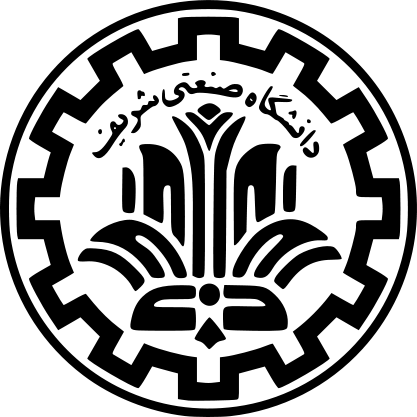
\includegraphics[width=1.6cm]{sharif.png}
\end{array}
$ \hspace{4.7cm} \textbf{اظهارنامه}
\small
\begin{center}
(اصالت متن و محتوای پایان‌نامه کارشناسی ارشد) \\
\end{center}
\vspace{0.5cm}
عنوان پایان‌نامه: 
\textbf{عنوان تز}
\\
نام استاد راهنما: 
\textbf{نام استاد راهنما}
 \hfill
نام استاد راهنمای همکار: 
\textbf{\ldots}
 \hfill
نام استاد مشاور: 
 \textbf{\ldots}
 \vspace{0.5cm}
 \\
 اینجانب \textbf{نام دانشجو} اظهار می‌دارم:
 \شروع{شمارش}
 \فقره متن و نتایج علمی ارائه‌شده در این پایان‌نامه اصیل بوده و منحصراً توسّط این‌جانب و زیر نظر استادان (راهنما، همکار و مشاور) نام‌برده شده در بالا تهیّه شده‌است.
 \فقره متن پایان‌نامه به این صورت در هیچ جای دیگری منتشر نشده‌است.
 \فقره متن و نتایج مندرج در این پایان‌نامه، حاصل تحقیقات این‌جانب به عنوان دانشجوی کارشناسی ارشد دانشگاه صنعتی شریف است.
 \فقره کلیه‌ی مطالبی که از منابع دیگر در این پایان‌نامه مورد استفاده قرار گرفته، با ذکر مرجع مشخّص شده‌است.
\پایان{شمارش}
\vspace{0.5cm}

\hspace{8cm} نام دانشجو: \textbf{نام دانشجو}

\hspace{8cm} تاریخ: \textbf{\today}

\hspace{8cm} امضاء:
\vspace{0.5cm}
\\
نتایج تحقیقات مندرج در این پایان‌نامه و دستاوردهای مادّی و معنوی ناشی از آن (شامل فرمول‌ها، توابع کتابخانه‌ای، نرم‌افزارها، سخت‌افزارها و مواردی که قابلیّت ثبت اختراع دارد) متعلّق به دانشگاه صنعتی شریف است. هیچ شخصیّت حقیقی یا حقوقی بدون کسب اجازه از دانشگاه صنعتی شریف حق فروش و ادعای مالکیّت مادّی یا معنوی بر آن یا ثبت اختراع از آن را ندارد. همچنین کلّیه‌ی حقوق مربوط به چاپ، تکثیر، نسخه‌برداری، ترجمه، اقتباس و نظائر آن در محیط‌های مختلف اعم از الکترونیکی، مجازی یا فیزیکی برای دانشگاه صنعتی شریف محفوظ است. نقل مطالب با ذکر مأخذ بلامانع است.

\vspace{0.5cm}
نام استاد راهنما: \textbf{نام استاد راهنما}
\hspace{2.9cm}
نام دانشجو: \textbf{نام دانشجو}

تاریخ: \textbf{\today}
\hspace{5.1cm}
تاریخ: \textbf{\today}

امضاء: 
\hspace{7cm}
امضاء: 

\normalsize

%تقدیم
\chapter*{}
\begin{center}
\vspace{0.9cm}
\large
\textbf{تقدیم}
\end{center}
تقدیم به پدر و مادر عزیزم.
%پیش‌گفتار
\chapter*{}
\begin{center}
\vspace{0.9cm}
\large
\textbf{پیش‌گفتار}
\end{center}
یک رساله خوب، بایستی پیش‌گفتاری زیبا و رسا داشته باشد.
%قدردانی
\chapter*{}
\begin{center}
\vspace{0.9cm}
\large
\textbf{قدردانی}
\end{center}
تشکر از استاد راهنما.
%چکیده فارسی
\chapter*{}
\begin{center}
\vspace{0.9cm}
\large
\textbf{چکیده}
\end{center}
چکیده اینجا قرار می‌گیرد.
\blfootnote{این فایل با مجوّز \lr{   (CC0-1.0)  } منتشر می‌گردد. \hfill
\includegraphics[width=1.8cm]{cc0.jpeg}}

\vspace{0.3cm}
\noindent\textbf{کلمات کلیدی:} چند کلمه‌ی کلیدی نمونه.

%فهرست‌ها
\tableofcontents \listoftables \listoffigures 

\pagebreak
\pagenumbering{arabic}
%شروع مطالب تز
%%%%%%%%%%%%%%%%%%%%%%%%%%%%%%%%%%%%%%%%%%%%%%%%
%مقدمه

\فصل{مقدمه و بیان مسأله}
\begin{itemize}
\item
موضوع کلّی
\item
سوال تحقیقاتی
\item
اهمیّت موضوع
\end{itemize}
%مرور ادبیات

\فصل{مرور ادبیات فنّی}
\label{lit_rev}
\begin{itemize}
\item
مرور تحقیقات گذشتگان
\item
ارتباط تحقیقات صورت‌گرفته و سوالات باقی‌مانده
\item
کاری که شما می‌خواهید انجام دهید
\item
سوالات باقی‌مانده از کار شما
\item
خلاصه‌ی سوال تحقیقاتی شما
\end{itemize}
%روش‌شناسی

\فصل{روش‌شناسی}
\label{method}
\begin{itemize}
\item
روش
\item
داده‌های مورد نیاز
\item
روش‌های آنالیز
\item
نحوه‌ی تفسیر نتایج
\end{itemize}

\قسمت{ارجاع به مقالات}
نمونه ارجاع به مقاله  \Latincite{Herbert1998}.

\قسمت{جدول}
جدول \ref{t1} نمونه یک جدول است.

\begin{center}
\begin{table}
\centering
\caption {‌جدول نمونه}
%\tabcolsep=0.12cm
\begin{tabular}{cr}
\hline 
متغیّر &  توضیح \\ \hline
$ Y $ &  سرانه‌ی ماحصل اقتصادی \\ 
$ I $ &  درآمد خالص اقتصادی \\ 
$ B $ &  نرخ زاد ولد \\ 
$ D $ &  نرخ مرگ‌ و میر \\ 
$ N $ &  جمعیّت \\ 
$ F $ &  جریان آلاینده‌ها \\ 
$ K $ &  منابع طبیعی \\ 
$ C $ &  هزینه‌ی صرف‌شده برای حفظ محیط‌زیست \\ 
$ P $ &  میزان آلودگی \\  \hline 
\end{tabular}
\label{t1}
\end{table}
\end{center}

\قسمت{تصویر}
شکل \ref{f1} نمونه‌ای از یک تصویر است.

\begin{figure}%[h]
	\centering
	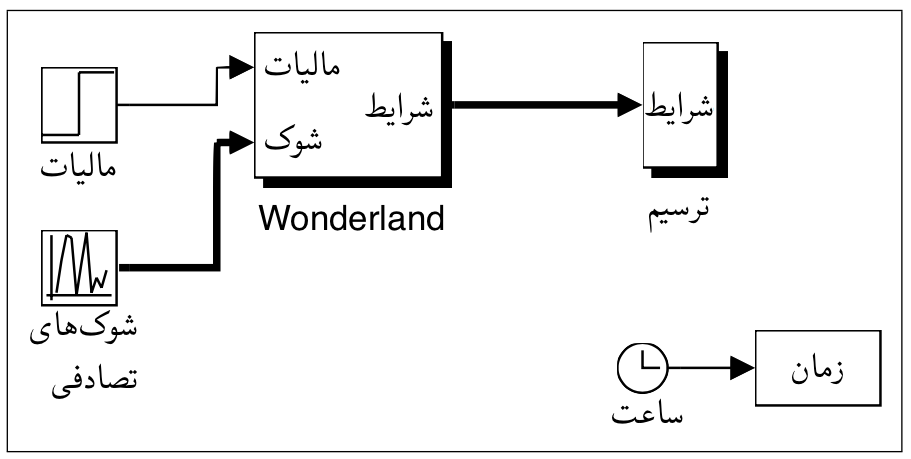
\includegraphics[width=12cm]{Wonderland.png}
	\caption{تصویر نمونه}
	\label{f1}
\end{figure}

\قسمت{معادلات ریاضی}
معادله \ref{e1} نمونه‌ای از یک رابطه ریاضی است.
\begin{equation}
	\label{e1}
	K_{t+1}= \frac{e^{ln(\frac{K_t}{1-K_t}+\delta K_t^\rho - \omega F_t)}}{1+e^{ln(\frac{K_t}{1-K_t}+\delta K_t^\rho - \omega F_t)}}
\end{equation}
 
 
%نتایج

\فصل{نتایج}
\label{results}
نتایج تز
%نتیجه‌گیری
\فصل{بحث و نتیجه‌گیری}
\label{conclusion}

%پیوست
\appendix

\فصل{پیوست}
\label{python}
نمونه‌ای از پیوست شامل کدهای یک برنامه‌ی فرترن.

\begin{latin}
\lstset{language=Fortran}
\begin{lstlisting}[frame=single, basicstyle=\footnotesize, numbers=left,breaklines=true]
print *, "Hello World!"
end
\end{lstlisting}
\end{latin}


%%%%%%
%مراجع
\lhead{}
%\renewcommand{\bibname}{\rl{{مراجع‌}}}‎
\bibliographystyle{asa-fa}
\bibliography{refs}

%%%%%%%%%
%English Abstract
\begin{latin}
\chapter*{}
\begin{center}
\vspace{0.9cm}
\large
\textbf{Abstract}
\end{center}
Abstract goes here.

\vspace{0.3cm}
\noindent\textbf{Key Words: }  Some keywords. 


%%%%%%%%%%
%English Title Page
\begin{titlepage}
\vspace*{1cm}
\begin{center}
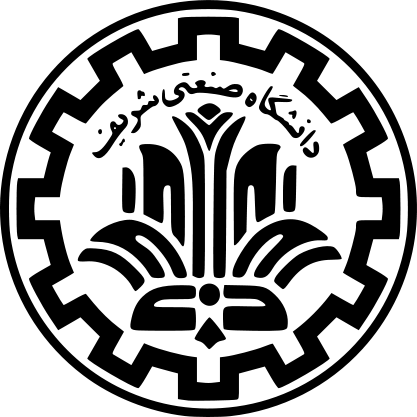
\includegraphics[width=4cm]{sharif.png}

 \large
Sharif University of Thechnology


Faculty of Civil Engineering

\vspace*{1cm}
\large
\textbf{A thesis submitted in partial fulfilment of the requirement for the M.Sc.~degree}


\textbf{Environmental Engineering}

\vspace*{1.5cm}
\Huge
\textbf{Thesis Title}     
\vspace{1.5cm}

\Large

By:

\textbf{Name}
\vspace{1.5cm}

Supervisor:

\textbf{Dr.~Supervisori}
\vfill
\Large
\latintoday        
\end{center}
\end{titlepage}

\end{latin}
\پایان{نوشتار}